\section{Slagterieksempel}
\fxnote{mere intro -  Rasmus hjælp}
Til at illustrere brugen af RTP vil vi illustrere et  problem fra Danish Crown slagteriet, der skal  udvikle er en beslutningsmodel, for hvordan en robot skal  udskære hver gris. På Danish Crown slagteriet i Horsens foretages udskæringen  grise som beskrevet på deres hjemmeside:

\begin{quote}\textit{``Grisen [\ldots] skal nu skæres i mindre, håndterbare stykker. Det sker i en meget avanceret maskine -- en såkaldt tredeler -- hvor hver halvdel af grisen deles i tre stykker: bov, mellemstykke og skinke. \\ 
\\
Robotten starter med at fotografere hver halvdel. Dataene fra billedet kombineres med ordren og kundens ønsker, hvorefter stykket deles i tre - nøjagtigt afpasset kundens ønsker.''}{ Danish Crowns hjemmeside\footnote{\url{http://www.danishcrown.dk/custom/horsens/3772.asp}}}\end{quote}

Et billede af den automatiske tredeler er vist  på \cref{fig:pig}.  Det har dog vist sig at udskæringen ikke  altid resulterer i en  optimal udskæring, da  ca. 10\% af alle grise har et ekstra sæt ribben som der ikke tages højde for. Til at løse dette problem har slagteriet udviklet skal robotten kunne bestemme om grisen har et ekstra st ribben inden den foretager udskæringen.

\begin{figure}
 \begin{center}
  \includegraphics[scale=0.5]{images/209690-1}
	\caption{Billedet viser i forgrunden  et foto taget af tredeleren til brug for analyse. I baggrunden ses transportbåndet, hvor de halve  grise venter på på at blive udskåret af den automatisk tredeler.}
	\label{fig:pig}
\end{center}
\end{figure}


Slagteriet har placeret kameraet i starten af et transportbåndet mens udskæringsrobotten findes i den anden enden. Der kan være flere svin på transportbåndet på samme tid, og det fremføre svinene i et fast tempo. Dette giver et fast tidsrum fra svinet passere kameraet til det passere robotten. Vi har hermed et klassisk RTP system, hvor robotten skal foretage et valg under en hard deadline, da der skal foretages en udskæring.

Vi må først se på arbejdsgangen der er involveret i valget af model:
\begin{enumerate}
\tightlist
	\item Et billede bliver taget af svinet mens den passere kameraet.
	\item Billedet konverteres til en 3D-model af svinet.
	\item 3D-modellen analyseres.
	\item Robotten udvælger hvor udskæringerne skal være på baggrund af analysen, ordren og kundens ønske.
	\item Robotten udskærer grisen.
\end{enumerate}

Man kan se at arbejdsgangen indeholder en  række klart afgrænsede arbejdsområder, som med fordel kan modelleres som selvstændige processer i \pycsp.  Vi har derfor valgt implementere følgende processer: Kamera, Billedekonvertering, 3D-analyse og en udvælgelse og udskæringsproces, hvilket leder til et procesnetværk som vist i \cref{fig:pig-network}.

\begin{figure}
 \begin{center}
  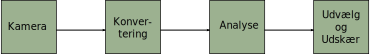
\includegraphics[scale=1]{images/pig-network}
	\caption{Procesnetværk til udskæring af svin på et slagteri.}
	\label{fig:pig-network}
\end{center}
\end{figure}

\subsubsection*{Implementering i \code{greenlets}-versionen}
Til at implementere eksemplet \code{greenlets}-versionen, kan vi oprette hvert svin som et objekt og tilknytte en deadline. Nu kan hver proces evaluere om svinet har overskredet sin deadline, i det tilfælde fjerne svinet, og stoppe den videre behandling. Da der er ikke angivet hvordan hele processen startes,  antager vi der findes en form for detektor foran kameraet, der opfanger når et svin passerer og som dermed starter processen. 

Når detektoren starter hele processen, opretter den et svineobjektet som den sender til kameraprocessen, samt sender en kopi direkte til udvælgelse og udskæringsprocessen. Dermed ved processen at der ankommer et svin som den skal udskære, og hvis den inden deadline får en analyse af svinet, kan den træffe et begrundet valg om hvordan udskæringen skal foretages,  men hvis ikke denne analyse findes, bruges blot standardmodellen til at udskære grisen. \CRef{fig:pig-network2} viser det endelige  netværk, hvor detektoren er introduceret, og som sender data til hhv. kameraprocessen og til udvælgelse og udskæringsprocessen. 

\begin{figure}
 \begin{center}
  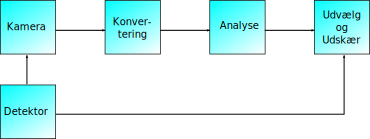
\includegraphics[scale=1]{images/pig-network2}
	\caption{Procesnetværk med detektor til initiering af hver gris.}
	\label{fig:pig-network2}
\end{center}
\end{figure}

Et problem ved at implementere  slagterieksemplet i \pycsp er  grænsefladen mellem verden hvor grisene kører på transportbåndet, og  \code{greenlets}-versionen.  I \pycsp  kan  kun en proces kan være aktiv af gangen og må arbejdet i  konvertering og analyse processen stoppe, mens  udskæringsprocessen foretager udskæringen. Konvertering- og analyseprocessen  skal dog frivilligt afgive kontrollen, mens svinet er indenfor robottens rækkevidden og hvis de ikke gør, bliver svinet ikke udskåret. Da dette er uacceptabelt ændrer vi systemet så det ikke er den samme applikation der både skal foretage alle tre processer. En applikation står for konvertering og analysen mens en anden  styrer robotten. De to applikationer skal dog kunne kommunikere, og  udveksle data, f.eks. igennem en database, harddisk eller anden delt datastruktur. Hvis analysen bliver færdig gemmes den, i den delte datastruktur, og robotten kan udnytte analysen, Hvis ikke den er klar bruges standardmodellen.    

Vi har holdt os tæt op af den virkelige verden, i designet af implementeringen, men da vi i sagens natur ikke har adgang til slagteriet og deres maskiner, eller præcis data om grisen, må vi nødvendigvis simulere dele af eksemplet. Man kan derfor se vores eksempel som rammen omkring processen og løbende som man får viden omkring de enkelte processer kan informationerne tilføjes de enkelte processer der dermed vil  give et stadigt mere præcist billede hvordan udskæringen vil forløbe. Detektoren er fuldstændigt simuleret, og indikerer at der ankommer en ny gris med et tilfældigt normalfordelt mellemrum. Da det er detektoren der står for oprettelsen objektet af grisen, som vi også simulere er det ved oprettelsen af grisen vi definere om den har et ekstra sæt ribben. 

Kamera, konvertering og analyse simulerer også kun bearbejdning af data. Hver proces modtager en gris, venter et normaltfordelt tidsrum der skal simulere dette arbejde og sender grisen videre. Udvælgelse og robot

Udvælgelse og udskærings processen reduceret til en IOproces der  modtager grisene og gemmer dem så en anden applikation kan tilgå dem.  til dette har vi valgt at bruge en \code{dictonary} dattastruktur til at gemme  hver gris under deres unikke id. Første gang processen modtager en gris gemmes den datastrukturen, så  tilfældet af analysen ikke bliver færdig vil den anden applikation som minimum vide der kommer en gris. Anden gang den samme gris ankommer er det fra analyseprocessen, med det færdige resultat. Processen overskriver den gamle gris, således den anden applikation, kan bruge den viden der er fundet igennem analysen.


%\subsection{Eksempel 2 - Sensornetværk med høj/lav -prioritet}
%\inline{eks2: skal vise alternation, kan være en sensor som modtager måledata med lav prioritet og som skal sende måledata på opdordring med høj prioritet.}
